\documentclass[aspectratio=169,10pt]{beamer}

\usetheme{Madrid}
\usecolortheme{dolphin}
\setbeamertemplate{navigation symbols}{}
\setbeamertemplate{footline}[frame number]

\usepackage[T1]{fontenc}
\usepackage[utf8]{inputenc}
\usepackage{booktabs}
\usepackage{array}
\usepackage{tabularx}
\usepackage{siunitx}
\usepackage{xcolor}
\usepackage{tikz}
\usetikzlibrary{positioning}
\usepackage{hyperref}

\definecolor{deepblue}{RGB}{30,74,108}
\definecolor{alertred}{RGB}{168,50,45}
\definecolor{softgreen}{RGB}{56,125,88}
\definecolor{warmgold}{RGB}{173,116,32}
\definecolor{mutedgray}{RGB}{92,99,108}
\definecolor{lightband}{RGB}{238,244,248}

\setbeamercolor{title}{fg=deepblue}
\setbeamercolor{frametitle}{fg=deepblue}
\setbeamercolor{structure}{fg=deepblue}
\setbeamercolor{alerted text}{fg=alertred}
\setbeamercolor{block title}{fg=white,bg=deepblue}
\setbeamercolor{block body}{bg=lightband}

\newcommand{\good}[1]{\textcolor{softgreen}{#1}}
\newcommand{\bad}[1]{\textcolor{alertred}{#1}}
\newcommand{\warn}[1]{\textcolor{warmgold}{#1}}
\newcommand{\muted}[1]{\textcolor{mutedgray}{#1}}
\newcommand{\mw}{\si{MW}}
\newcommand{\mvar}{\si{MVAr}}

\title[NPCC--NY Weekly Update]{NPCC--NY Lite Weekly Update}
\subtitle{Overvoltage repair, downstate delivery spine, generation alignment, and current tie-line mismatch}
\author{NPCC / NY-lite Calibration Workstream}
\date{July 8, 2026}

\begin{document}

\begin{frame}
  \titlepage
\end{frame}

\begin{frame}{This Week's Message}
\begin{block}{Status}
The model moved from an overvoltage / ACOPF-feasibility diagnosis to a working S4 calibration candidate.
\end{block}

\begin{itemize}
  \item The earlier public-load ACOPF failure was not mainly a branch-rating problem.
  \item Relaxed-voltage solves exposed a \bad{system-wide high-voltage escape path}, with all NY-only buses near 2.0 pu.
  \item The fix was not one more line alone: it required downstate delivery paths plus missing downstate active-power controllability.
  \item S3 restored feasibility with a bounded Zone J supply equivalent.
  \item S4 aligned zonal generation participation using Gold Book capability targets and improved interface behavior.
  \item Remaining problem: \warn{tie-line / interface residuals are still material}, especially Total East.
\end{itemize}
\end{frame}

\begin{frame}{Original Failure Mode}
\begin{columns}[T,onlytextwidth]
\begin{column}{0.48\linewidth}
\begin{block}{What failed}
\begin{itemize}
  \item Public NYISO load shapes were scaled to the preserved NPCC New York load level.
  \item Normal ACOPF failed under public downstate load relocation.
  \item Removing ratings alone did not restore ACOPF feasibility.
\end{itemize}
\end{block}
\end{column}
\begin{column}{0.48\linewidth}
\begin{block}{What the relaxed solve revealed}
\begin{itemize}
  \item ACOPF could solve only after voltage bounds were relaxed to 0.1--2.0 pu and ratings were removed.
  \item The optimizer drove the whole NY-only subsystem to abnormal high voltage.
  \item That made the relaxed solution a diagnostic, not a valid operating point.
\end{itemize}
\end{block}
\end{column}
\end{columns}

\vspace{0.5em}
\begin{center}
\small The core issue became: \textbf{AC voltage / controllability infeasibility under public load relocation}.
\end{center}
\end{frame}

\begin{frame}{Overvoltage Evidence}
\scriptsize
\begin{tabularx}{\linewidth}{X r r r}
\toprule
\textbf{Public scenario} & \textbf{$V_{\min}$} & \textbf{$V_{\max}$} & \textbf{Buses above 1.10 pu} \\
\midrule
Summer peak & 1.9534 & 2.0000 & 46 / 46 \\
Winter peak & 1.9483 & 2.0000 & 46 / 46 \\
Shoulder light load & 1.9449 & 2.0000 & 46 / 46 \\
High NYC / LI load & 1.9534 & 2.0000 & 46 / 46 \\
High Total East & 1.9453 & 2.0000 & 46 / 46 \\
Low Total East & 1.9478 & 2.0000 & 46 / 46 \\
\bottomrule
\end{tabularx}

\vspace{0.9em}
\begin{block}{Interpretation}
The overvoltage was not localized. It affected every retained NY bus in the relaxed diagnostic cases, including upstate, lower-Hudson, NYC proxy, and Long Island proxy buses.
\end{block}
\end{frame}

\begin{frame}{Main Causes of the Overvoltage Problem}
\begin{enumerate}
  \item \textbf{Public load relocation changed nodal stress.}\\
  Several GW moved toward G/J/K-style downstate proxy areas that had little or no original NPCC load.

  \item \textbf{The reduced topology lacked downstate delivery structure.}\\
  Initial paths could not represent the Central East $\rightarrow$ Total East $\rightarrow$ UPNY--ConEd $\rightarrow$ NYC / LI corridor sequence.

  \item \textbf{The boundary equivalent was exact only at S1.}\\
  Fixed measured boundary injections reproduced S1, but did not adapt like a dynamic external network under new public scenarios.

  \item \textbf{Voltage and reactive controls were too idealized.}\\
  Generator $Q$, boundary generator $Q$, branch charging, and unconstrained voltage objectives allowed abnormal voltage behavior when bounds were relaxed.

  \item \textbf{Missing local active-power controllability in Zone J.}\\
  The reduced model was forcing NYC public load to be served through coarse import paths with too little local equivalent supply.
\end{enumerate}
\end{frame}

\begin{frame}{Repair Strategy}
\begin{center}

\begin{tikzpicture}[node distance=0.35cm, every node/.style={font=\scriptsize}]
  \tikzstyle{box}=[rectangle, rounded corners=2pt, draw=deepblue, fill=lightband, text width=2.15cm, align=center, minimum height=0.9cm]
  \node[box] (s1) {S1 ACOPF feasible base};
  \node[box, right=of s1] (eq) {NY-only boundary equivalent};
  \node[box, right=of eq] (spine) {S2 downstate delivery spine};
  \node[box, right=of spine] (j) {S3 Zone J supply equivalent};
  \node[box, right=of j] (s4) {S4 Gold Book generation alignment};
  \draw[->, thick, deepblue] (s1) -- (eq);
  \draw[->, thick, deepblue] (eq) -- (spine);
  \draw[->, thick, deepblue] (spine) -- (j);
  \draw[->, thick, deepblue] (j) -- (s4);
\end{tikzpicture}
\end{center}

\vspace{0.8em}
\begin{itemize}
  \item S1: replace embedded infeasible dispatch with an ACOPF-feasible base point.
  \item NY-only equivalent: remove external NPCC branch dominance while preserving measured S1 boundary behavior.
  \item S2: add no-load downstate transit paths with zero added branch charging initially.
  \item S3: add bounded aggregate NYC / Zone J active supply.
  \item S4: align zonal capability and participation to public NYISO Gold Book patterns.
\end{itemize}
\end{frame}

\begin{frame}{S2: Downstate Delivery Spine}
\small
\begin{center}
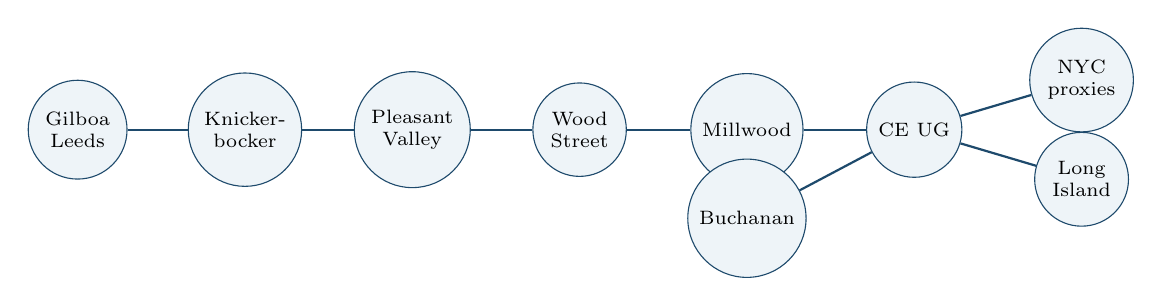
\begin{tikzpicture}[x=1.25cm,y=0.9cm, every node/.style={font=\scriptsize}]
  \tikzstyle{zonebox}=[circle, draw=deepblue, fill=lightband, minimum size=0.82cm, align=center]
  \node[zonebox] (gl) at (0,0) {Gilboa\\Leeds};
  \node[zonebox] (kb) at (1.7,0) {Knicker-\\bocker};
  \node[zonebox] (pv) at (3.4,0) {Pleasant\\Valley};
  \node[zonebox] (ws) at (5.1,0) {Wood\\Street};
  \node[zonebox] (mw) at (6.8,0) {Millwood};
  \node[zonebox] (ce) at (8.5,0) {CE UG};
  \node[zonebox] (nyc) at (10.2,0.7) {NYC\\proxies};
  \node[zonebox] (li) at (10.2,-0.7) {Long\\Island};
  \node[zonebox] (buch) at (6.8,-1.25) {Buchanan};
  \draw[thick, deepblue] (gl) -- (kb) -- (pv) -- (ws) -- (mw) -- (ce);
  \draw[thick, deepblue] (buch) -- (ce);
  \draw[thick, deepblue] (ce) -- (nyc);
  \draw[thick, deepblue] (ce) -- (li);
  \draw[thick, deepblue] (mw) -- (ce);
\end{tikzpicture}
\end{center}

\vspace{0.5em}
\begin{itemize}
  \item Added zero-load transit buses: Knickerbocker, Wood Street, East Garden City.
  \item Added delivery paths toward Pleasant Valley, Millwood, CE UG, NYC proxies, and Northport.
  \item Initial new-line parameters used high ratings and $B_c = 0$ to avoid adding more capacitive charging.
  \item Result: improved public active-load continuation boundary, but did \bad{not} make full public relocation feasible by itself.
\end{itemize}
\end{frame}

\begin{frame}{S3: Missing Zone J Active-Power Equivalent}
\begin{columns}[T,onlytextwidth]
\begin{column}{0.49\linewidth}
\begin{block}{Why it was needed}
\begin{itemize}
  \item Public load relocation placed several GW into NYC proxy buses.
  \item Real NYISO Zone J has substantial local capability.
  \item The reduced NPCC mapping had proxy buses but lacked sufficient local controllable active supply.
\end{itemize}
\end{block}
\end{column}
\begin{column}{0.49\linewidth}
\begin{block}{Implementation}
\begin{itemize}
  \item Added bounded aggregate supply at RAV A-3, AK-3, and Goethals.
  \item Interpreted as NYC local generation / import equivalent, not unit-level modeling.
  \item Default working cap: 3.0 GW.
\end{itemize}
\end{block}
\end{column}
\end{columns}

\vspace{0.7em}
\scriptsize
\begin{tabularx}{\linewidth}{X r r r}
\toprule
\textbf{Zone J PMAX test} & \textbf{Cases} & \textbf{Successes} & \textbf{Max Zone J dispatch} \\
\midrule
No Zone J equivalent & 6 & 0 & 0 MW \\
2.40 GW threshold & 6 & 5 & 2400 MW \\
2.45 GW threshold & 6 & 6 & 2431 MW \\
3.00 GW default & 6 & 6 & 2430 MW \\
\bottomrule
\end{tabularx}
\end{frame}

\begin{frame}{Voltage Issue After S3}
\begin{itemize}
  \item S3 restored normal-bound ACOPF feasibility for public P-only, public Q-only, public P+Q, and public P+Q plus public external schedule tests.
  \item The 3.0 GW Zone J equivalent was not binding in the broad S3 validation set.
  \item The previous 2.0 pu escape was eliminated from the accepted operating cases.
  \item Remaining voltage issue is now milder but still visible: many S4 OPFs sit on 0.90 / 1.10 pu bounds.
\end{itemize}

\vspace{0.6em}
\begin{block}{Updated interpretation}
S3 solved the \textbf{feasibility and abnormal-overvoltage} problem, but did not yet calibrate the interface-flow behavior.
\end{block}
\end{frame}

\begin{frame}{Gold Book Generation Alignment}
\scriptsize
\begin{tabularx}{\linewidth}{l r X}
\toprule
\textbf{Zone} & \textbf{2025 Gold Book summer capability} & \textbf{Modeling implication} \\
\midrule
A -- WEST & 3492.4 MW & Existing NPCC/S3 participation was too high; cap participation. \\
B -- GENESE & 780.5 MW & Existing NPCC/S3 participation was too high; cap participation. \\
C -- CENTRL & 6781.1 MW & Large resource zone, but still avoid excessive upstream export. \\
F -- CAPITL & 4775.6 MW & Add / enable Capital-region equivalent capability. \\
G -- HUD VL & 4704.0 MW & Add Hudson Valley equivalent capability near lower-Hudson proxies. \\
I -- DUNWOD & 0.0 MW & Reclassify CE UG as interface / voltage support, not native Zone I generation. \\
J -- N.Y.C. & 8704.7 MW & Keep bounded Zone J aggregate supply equivalent. \\
K -- LONGIL & 5195.5 MW & Add Long Island equivalent capability near Northport / East Garden City. \\
\bottomrule
\end{tabularx}

\vspace{0.4em}
\footnotesize Source values are from the local project Gold Book target table used for S4 generation alignment.
\end{frame}

\begin{frame}{S4 Model Changes}
\begin{columns}[T,onlytextwidth]
\begin{column}{0.5\linewidth}
\begin{block}{Added capability}
\begin{itemize}
  \item E: Edic / Porter equivalent.
  \item F: Gilboa, Albany, Rotterdam, New Scotland equivalents.
  \item G: Pleasant Valley, Ramapo, Leeds equivalents.
  \item K: Northport and East Garden City equivalents.
\end{itemize}
\end{block}
\end{column}
\begin{column}{0.5\linewidth}
\begin{block}{Participation controls}
\begin{itemize}
  \item A/B/C participation caps, best candidates use factor 0.8.
  \item CE UG generator moved away from native Zone I role.
  \item Relative costs tune Zone J vs non-J equivalent participation.
  \item Spine $X$ sensitivity was secondary to participation alignment.
\end{itemize}
\end{block}
\end{column}
\end{columns}

\vspace{0.6em}
\begin{center}
\small Final S4 candidate cases reload as \textbf{143 buses, 246 branches, 62 generators}.
\end{center}
\end{frame}

\begin{frame}{Optimization Problem: Inner ACOPF}
\small
For each public scenario $s$ and candidate parameter set $\theta$, the solved problem is the MATPOWER ACOPF:
\vspace{-0.2em}
\scriptsize
\begin{align*}
\min_{x_s}\quad
& \sum_{g \in \mathcal{G}}
\left(c_{2g}P_{g,s}^2 + c_{1g}P_{g,s} + c_{0g}\right)
+ \rho_V \sum_{i \in \mathcal{B}} (V_{i,s}-V_i^{ref})^2 \\[0.25em]
\text{s.t.}\quad
& g_i^P(\theta_s,V_s,P_s,Q_s)=0,\qquad
  g_i^Q(\theta_s,V_s,P_s,Q_s)=0 \\
& P_g^{min} \le P_{g,s} \le P_g^{max},\qquad
  Q_g^{min} \le Q_{g,s} \le Q_g^{max} \\
& V_i^{min} \le V_{i,s} \le V_i^{max} \\
& |S_{\ell,s}^{from}| \le RATE_{A,\ell},\qquad
  |S_{\ell,s}^{to}| \le RATE_{A,\ell}.
\end{align*}

\normalsize
\begin{itemize}
  \item Public P-58C load and P-32 external schedules are fixed inputs for scenario $s$.
  \item S3/S4 equivalent-resource costs and limits enter through $c_g$, $P_g^{min}$, and $P_g^{max}$.
  \item Interface-flow matching is \textbf{not} embedded in this inner ACOPF yet.
\end{itemize}
\end{frame}

\begin{frame}{Outer Calibration Problem}
\small
The calibration variables are candidate parameters rather than bus voltages directly:
\[
\theta =
\{c_{1,J}, c_{1,E}, c_{1,F}, c_{1,G}, c_{1,K},
\alpha_{ABC}, X_{\mathrm{spine}}, P^{max}_{J,eq}\}.
\]

\vspace{-0.4em}
\begin{block}{Current implemented workflow}
\[
\theta \rightarrow
\text{build S4 candidate cases} \rightarrow
\text{solve IPOPT ACOPF for all scenarios} \rightarrow
\text{score interface residuals}.
\]
\end{block}

\vspace{-0.2em}
\scriptsize
\begin{align*}
\theta^\star
&= \arg\min_{\theta \in \Theta}
J_{\mathrm{cal}}(\theta) \\
J_{\mathrm{cal}}(\theta)
&= \sum_{s \in \mathcal{S}} J_{\mathrm{int}}(\theta;s)
\quad \text{subject to OPF success and no branch-overload rejection.}
\end{align*}

\normalsize
\begin{itemize}
  \item The grid search tested 178 candidate settings and 1,068 IPOPT ACOPFs.
  \item All reported S4 candidate objective values are \textbf{post-OPF interface scores}, not the raw MATPOWER generation-cost objective.
\end{itemize}
\end{frame}

\begin{frame}{Interface Objective Used for Candidate Ranking}
\small
For each scenario $s$ and monitored interface $m$:
\[
e_{s,m}(\theta)
=
F_{s,m}^{lite}(\theta)-F_{s,m}^{target}.
\]

\vspace{-0.2em}
\begin{columns}[T,onlytextwidth]
\begin{column}{0.48\linewidth}
\begin{block}{Classic score}
\scriptsize
\[
J_{\mathrm{classic}}(\theta)
=
\sum_{s,m}
\left[
\frac{e_{s,m}(\theta)}
{\max(100,\ |F_{s,m}^{target}|)}
\right]^2.
\]
\end{block}
\end{column}
\begin{column}{0.48\linewidth}
\begin{block}{Fixed-scale score}
\scriptsize
\[
J_{\mathrm{fixed}}(\theta)
=
\sum_{s,m}
\left[
\frac{e_{s,m}(\theta)}
{S_m^{fixed}}
\right]^2.
\]
\[
S_m^{fixed}=\max(500,\ \widetilde{L}_m^{P32,scaled}).
\]
\end{block}
\end{column}
\end{columns}

\vspace{0.4em}
\begin{itemize}
  \item The fixed-scale score uses one stable scale per interface from the median available scaled P-32 limit.
  \item It avoids over-weighting low-flow or missing-limit rows with an artificial 500 MW fallback.
  \item The current v2 candidate is selected by $J_{\mathrm{fixed}}$.
\end{itemize}
\end{frame}

\begin{frame}{S4 Calibration Results}
\footnotesize
Objective values below are post-OPF interface scores accumulated across six public scenarios.

\vspace{0.4em}
\scriptsize
\begin{tabularx}{\linewidth}{X r r r r}
\toprule
\textbf{Case} & \textbf{Success} & \textbf{Classic obj.} & \textbf{Mean Zone J eq.} & \textbf{Mean S4 non-J eq.} \\
\midrule
S3 baseline, 3.0 GW Zone J & 6 / 6 & 893.20 & 1443 MW & 0 MW \\
S4 equivalents only & 6 / 6 & 910.11 & 0 MW & 2035 MW \\
S4 equivalents + A/B/C caps & 6 / 6 & 312.50 & 0 MW & 2767 MW \\
Cost sweep v1, classic-best style & 6 / 6 & 93.52 & 2861 MW & 649 MW \\
Cost sweep v2, fixed-scale best & 6 / 6 & 132.03 & 1392 MW & 2151 MW \\
\bottomrule
\end{tabularx}

\vspace{0.7em}
\begin{block}{Key point}
Generation participation and cost alignment produced the largest improvement. Topology-only changes were necessary, but not sufficient.
\end{block}
\end{frame}

\begin{frame}{Candidate Choice Depends on Scoring Basis}
\footnotesize
Both columns are post-OPF residual objectives: $J_{\mathrm{classic}}$ and $J_{\mathrm{fixed}}$, not separate ACOPF objective functions.

\vspace{0.35em}
\scriptsize
\begin{tabularx}{\linewidth}{X r r r r}
\toprule
\textbf{Candidate} & \textbf{Classic obj.} & \textbf{Fixed-scale obj.} & \textbf{Mean Zone J} & \textbf{Mean S4 non-J} \\
\midrule
v1: J220 / EFGK260 / CAP0.8 / X1 & \good{93.52} & 7.728 & 2861 MW & 649 MW \\
v2: J180 / EFGK180 / CAP0.8 / X1 & 132.03 & \good{4.335} & 1392 MW & 2151 MW \\
\bottomrule
\end{tabularx}

\vspace{0.7em}
\begin{itemize}
  \item v1 remains the better classic-objective candidate and uses more Zone J supply.
  \item v2 is preferred after correcting interface normalization with fixed interface scales.
  \item The corrected fixed-scale objective avoids over-weighting missing P-32 limits with a 500 MW fallback.
  \item Current recommendation: use v2 as the fixed-scale S4 candidate; keep v1 as a Zone-J-heavy sensitivity.
\end{itemize}
\end{frame}

\begin{frame}{Current Tie-Line / Interface Mismatch}
\scriptsize
\begin{tabularx}{\linewidth}{X r r r}
\toprule
\textbf{Interface} & \textbf{Fixed scale} & \textbf{Mean abs. residual} & \textbf{Max abs. residual} \\
\midrule
Total East proxy & 2905 MW & 938 MW & 1800 MW \\
Central East & 1393 MW & 651 MW & 751 MW \\
Moses South & 1125 MW & 459 MW & 605 MW \\
UPNY--ConEd & 2999 MW & 437 MW & 1655 MW \\
Dunwoodie South & 1936 MW & 411 MW & 1413 MW \\
\bottomrule
\end{tabularx}

\vspace{0.7em}
\begin{block}{Interpretation}
The remaining problem is not raw ACOPF feasibility or branch overload. It is behavioral mismatch: the reduced tie-line and generation-equivalent model still does not reproduce all scaled P-32 interface patterns.
\end{block}
\end{frame}

\begin{frame}{Why Mismatch Remains}
\begin{itemize}
  \item P-32 interface flows are aggregate system outcomes, not individual branch ratings.
  \item S4 still uses reduced proxy corridors and equivalent generators instead of detailed NYISO internal topology.
  \item Zone J vs G/K/F/E equivalent dispatch shifts the burden between local supply and upstream imports.
  \item Total East remains sensitive to A/B/C participation, F/G supply, and Gilboa--Leeds / downstate-spine reactance.
  \item UPNY--ConEd and Dunwoodie South remain sensitive to how much NYC load is served locally versus through lower-Hudson paths.
\end{itemize}

\vspace{0.5em}
\begin{center}
\small The mismatch is now a calibration problem, not an overvoltage rescue problem.
\end{center}
\end{frame}

\begin{frame}{Next Work Items}
\begin{enumerate}
  \item \textbf{Refine the fixed-scale S4 candidate.}\\
  Sweep near v2: Zone J and S4 equivalent costs around 180--220, A/B/C cap factor around 0.75--0.85, and $X$ at 1.0 / 0.75.

  \item \textbf{Report dispatch plausibility.}\\
  Track Zone J, F, G, K, E, and A/B/C generation by scenario so equivalents do not become hidden slack resources.

  \item \textbf{Add voltage-deviation diagnostics.}\\
  Voltage penalty reduced bound hits in v1 tests, but did not eliminate them.

  \item \textbf{Prototype exact AC interface objective later.}\\
  Do not fake interface flow penalties as linear generalized costs; exact AC branch-flow penalties should use nonlinear-cost callbacks.

  \item \textbf{Keep holdout scenarios.}\\
  Candidate selection should be tested on scenarios not used for tuning.
\end{enumerate}
\end{frame}

\begin{frame}{Takeaways}
\begin{itemize}
  \item The old relaxed-voltage solution identified a true modeling issue: public-load cases could escape to system-wide 2.0 pu voltages.
  \item S2 added missing downstate delivery structure but was not enough on its own.
  \item S3 fixed the main feasibility problem by adding bounded NYC / Zone J active-power controllability.
  \item S4 aligned generation capability and participation using Gold Book zonal patterns, giving a much stronger calibration candidate.
  \item The present limitation is tie-line and interface-flow mismatch, especially Total East, not ACOPF convergence.
\end{itemize}

\vspace{0.7em}
\begin{block}{Current status}
\textbf{Feasible and materially improved; still candidate-level interface calibration.}
\end{block}
\end{frame}

\begin{frame}{Local Artifacts}
\scriptsize
\begin{tabularx}{\linewidth}{l X}
\toprule
\textbf{Artifact} & \textbf{Role} \\
\midrule
\texttt{npcc\_ny\_lite\_s4\_cost\_calibration\_candidate\_v2.m} & Fixed-scale S4 candidate case. \\
\texttt{s4\_cost\_penalty\_fixed\_scale\_rescore\_summary.csv} & Corrected fixed-scale candidate ranking. \\
\texttt{s4\_candidate\_validation\_combined\_20260703\_212010.zip} & Combined S4 candidate validation archive. \\
\texttt{nyiso\_interface\_objective\_scales.csv} & Fixed interface normalization scales. \\
\texttt{ny\_only\_case\_d\_vmax2\_overvoltage\_buses.csv} & Relaxed-voltage overvoltage evidence. \\
\bottomrule
\end{tabularx}

\vspace{0.7em}
\begin{center}
\footnotesize All results shown here are from local MATPOWER/IPOPT runs and project CSV outputs.
\end{center}
\end{frame}

\end{document}
